% Created 2016-02-15 Mon 08:53
\documentclass[11pt]{article}
\usepackage[utf8]{inputenc}
\usepackage[T1]{fontenc}
\usepackage{fixltx2e}
\usepackage{graphicx}
\usepackage{grffile}
\usepackage{longtable}
\usepackage{wrapfig}
\usepackage{rotating}
\usepackage[normalem]{ulem}
\usepackage{amsmath}
\usepackage{textcomp}
\usepackage{amssymb}
\usepackage{capt-of}
\usepackage{hyperref}
\usepackage{tikz}
\usepackage{fancyhdr}
\usepackage[left=2cm,right=2cm,top=2cm,bottom=2cm]{geometry}
\renewcommand\vec{\mathbf}
\newcommand\leftidx[3]{{\vphantom{#2}}#1#2#3}
\newenvironment{example}[1]{\vspace{0.2in}\hrule\vspace{0.1in}\noindent\emph{Example:} #1 \\}{\vspace{0.1in}\hrule\vspace{0.2in}}
\pagestyle{fancyplain}
\cfoot{{\it ENGY 5050, Nuclear Reactor Physics, UMass Lowell}}
\author{Justin Pounders}
\date{\today}
\title{Neutron Slowing Down}
\hypersetup{
 pdfauthor={Justin Pounders},
 pdftitle={Neutron Slowing Down},
 pdfkeywords={},
 pdfsubject={},
 pdfcreator={Emacs 24.5.1 (Org mode 8.3.2)}, 
 pdflang={English}}
\begin{document}

\maketitle
\tableofcontents

\section{Energy balance equation}
\label{sec:orgheadline1}
If we assume that a reactor is very large with respect to the mean free path of a neutron and consists of a homogeneous material then we may write a balance equations for the neutron density with respect to energy.  In reality, spatial effects will play a role in determining the neutron density, but we will consider those later.  Describing the neutron density with respect to energy alone unveils some important aspects of reactor physics.  The neutron balance equation for neutrons with energy between \(E\) and \(E+dE\) is
\begin{align}
  \left[ \Sigma_a(E) + \Sigma_s(E) \right] \phi(E) dE
  = \left[ \int_0^\infty dE' \Sigma_s(E' \rightarrow E ) \phi(E')
           + \frac{\chi(E)}{k_\infty} \int_0^\infty dE' \nu\Sigma_f(E') \phi(E') \right] dE
\end{align}
where \(\Sigma_a(E)\) is the macroscopic absorption cross section, \(\Sigma_s(E)\) is the macroscopic scattering cross section, \(\Sigma_s(E' \rightarrow E)\) is the scattering kernel (i.e., \(\Sigma_s(E)\) multiplied by the probability of a scattering event changing a neutron's energy from \(E'\) to \(E\)), and \(\Sigma_f(E)\) is the macroscopic fission cross section.  Additionally, \(\chi(E)\) is the \emph{fission spectrum}, which represents the probability that a neutron emitted from fission will emerge with an energy \(E\), and \(\nu\) is the average number of neutrons released per fission.  The factor \(k_\infty\) is the \emph{infinite multiplication factor}, which is needed to ensure a steady-state solution for the scalar flux, \(\phi(E)\).

It is presumed that all cross sections and fission parameters are known.  Our present goal is then to solve the neutron balance equation for the energy-dependent flux \(\phi(E)\).  Note that this equation is not an ``energy balance'' equation in the sense that it balances the neutron kinetic energy.  Rather, it balances the number of neutrons with a given kinetic energy, namely \(n(E)dE\), which is the number of neutrons between \(E\) and \(E+dE\).  The function \(\phi(E)\), where \(E\) is the only independent variable, is often called the \emph{neutron spectrum}.

\section{Characteristic Neutron Energy Ranges}
\label{sec:orgheadline5}
Rather than seeking an immediate solution to this neutron balance equation, we will first conduct a qualitative exploration of solution.  Neutrons are created from fission with a relatively high kinetic energy, yet the fission cross section tends to be highest at lower (thermal) energies, as shown in Figure \ref{fig::u235fission}.  In between there are large discrete capture resonances that the neutrons must escape while slowing down to thermal energies.
\begin{figure}
  \centering
  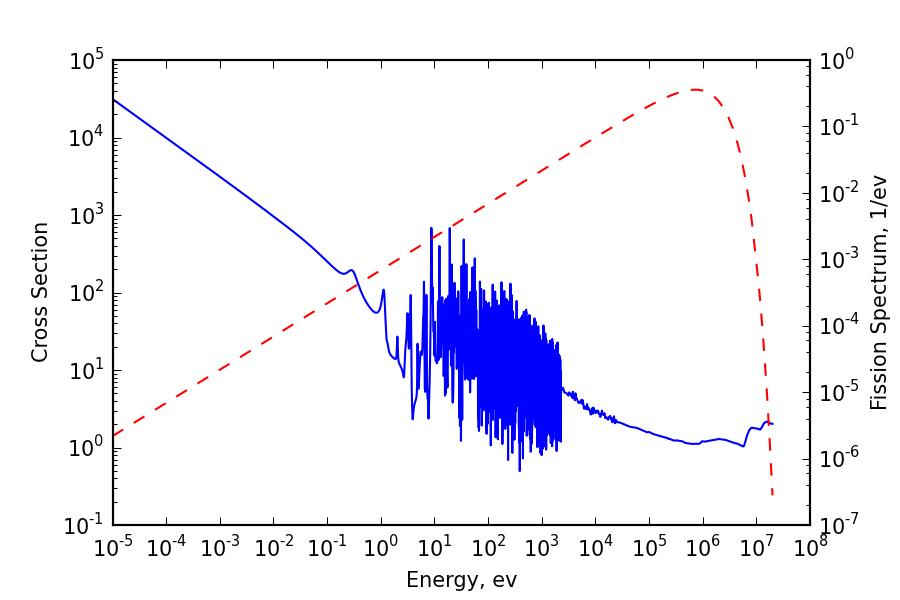
\includegraphics[width=0.75\textwidth]{u235fission.png}
  \caption{Fission cross section (blue) and fission spectrum (red) of uranium-235.}
  \label{fig::u235fission}
\end{figure}

These three energy ranges (fission spectrum, slowing down, and thermal) each impact the neutron spectrum, \(\phi(E)\), in qualitatively different ways.  We can roughly characterize the spectrum in each range by introducing some approximations that permit an analytical solution to the neutron balance equation.
\subsection{Fission Energy Range}
\label{sec:orgheadline2}
Neutrons are typically emitted from fission with a kinetic energy of 1 to 2 MeV.  This is much higher than the thermal equilibrium energy that is on the order of 1 eV.  At these high energies, the rate of neutrons being created in interval \(dE\) from fission is much greater than neutrons being scattered into \(dE\) from lower energies.  Thus
\begin{align}
  \phi(E) dE \approx  \frac{\chi(E)}{k_\infty\Sigma_t(E)} \int_0^\infty dE' \nu\Sigma_f(E') \phi(E')  dE = \frac{\chi(E)}{\Sigma_t(E)} \times \text{ constant}.
\end{align}
Thus the neutron spectrum at high energies, say \(E > 0.5 MeV\), is roughly proportional to the fission spectrum divided by the total cross section.

The fission spectrum can be described by a number of different formulations, one of which is the Watt spectrum.  The Watt spectrum is a probability density that can be written
\begin{align}
  p_\text{Watt}(E) = \frac{1}{I} \sinh\sqrt{bE} e^{-E/a}
\end{align}
where \(I\) is a normalization constant, and \(a\) and \(b\) are parameters.  For uranium-235,
\begin{align}
  I &= 2.0555, \\
  a &= 1, \\
  b &= 2,
\end{align}
for \(E\) in MeV.  Integrating this function reveals that roughly 88\% of neutrons are created with an energy between 0.1 and 4 MeV, and only 1.4\% are created with an energy \emph{less} than 0.1 MeV.  The average energy is 2 MeV and the median is about 1.6 MeV.

\subsection{Slowing-Down Energy Range}
\label{sec:orgheadline3}
At energies between 1 eV and 50 keV, there are very few neutrons created directly from fission and elastic scattering is much more important than inelastic scattering.  (Why?)  The elastic scattering cross kernel can be written
\begin{align}
  \Sigma_s(E' \rightarrow E) = 
  \begin{cases}
    \frac{\Sigma_s(E')}{E'(1-\alpha)}, & E \leq E' \leq \frac{E}{\alpha} \\
    0, & \text{otherwise}
  \end{cases}
\end{align}
where \(\alpha = \left[(A-1)/(A+1)\right]^2\).  If there are \(J\) nuclides present then the neutron balance equation becomes
\begin{align}
  \Sigma_t(E) \phi(E) dE
  = \sum_{j=1}^J \left[ \int_E^{E/\alpha_j} dE' \frac{\Sigma_s(E')}{E'(1-\alpha)} \phi(E') \right] dE.
\end{align}

Let's consider the case of neutron slowing down in the presence of hydrogen plus large resonance aborbers.  If the \(j=1\) nuclide is hydrogen (\(\alpha=0\)) and all the others are quite heavy (\(\alpha \approx 1\)) then we can write
\begin{align}
  \Sigma_t(E) \phi(E)
  &=  \left[ \int_E^\infty dE' \frac{\Sigma_s^H(E')}{E'} \phi(E') \right]
    + \sum_{j=2}^J \left[ \int_E^{E/\alpha_j} dE' \frac{\Sigma_s^j(E')}{E'(1-\alpha)} \phi(E') \right] \\
  &\approx  \int_E^\infty dE' \frac{\Sigma_s(E')}{E'} \phi(E')
    + \sum_{j=2}^J \frac{\Sigma_s(E)}{\alpha} \phi(E) 
\end{align}
where in the second approximation we have used \(\Sigma_s^j(E')\phi(E')/E' \approx \Sigma_s^j(E)\phi(E)/E\) for \(E' \in [E, E/\alpha_j]\).  This equation can be manipulated to yield (approximately
\begin{align}
  \left[ \Sigma_a(E) + \Sigma_s^H(E) \right] \phi(E)
  &= \int_E^\infty dE' \frac{\Sigma_s^H(E')}{E'} \phi(E')
\end{align}
where on the left-hand-side we have used \(\Sigma_s^H(E) \approx \Sigma_s(E) - \sum_{j=2}^J \Sigma_s^j(E)/\alpha\).  Differentiating this expression and defining a new function \(f(E) = \left[ \Sigma_a(E) + \Sigma_s^H(E) \right] \phi(E)\) leads to
\begin{align}
  \frac{df}{dE} &= - \frac{\Sigma_s^H(E)}{E\left[ \Sigma_a(E) + \Sigma_s^H(E) \right]} f(E).
\end{align}
This equation can be solved using an integrating factor and integrating from \(E\) to some arbitrary energy \(E_1\), ultimately leading to
\begin{align}
  \phi(E) = \frac{\left[ \Sigma_a(E_1) + \Sigma_s^H(E_1) \right] E_1 \phi(E_1)}{\left[ \Sigma_a(E) + \Sigma_s^H(E) \right] E}
            \exp\left[ -\int_E^{E_1} \frac{\Sigma_a(E')}{\left[ \Sigma_a(E') + \Sigma_s^H(E') \right] E'} dE' \right].
\end{align}
Thus \(\phi(E)\) varies fundamentally as \(1/E\) with localized perturbations caused by resonances that manifest in \(\Sigma_a(E)\) in the denominator of the first term and an overall attenuation arising from the exponential term, which again is primarily affected by resonances along the energy path from \(E_1\) to \(E\).

The fact that the flux will be locally depressed in the vicinity of a large absorption resonance is called \emph{energy self-shielding}.  The name suggests that because the neutron population is suppressed in a resonance energy range, the neutrons are naturally ``shielded'' from the resonance to some degree.

A rough estimate of the number of neutrons that will be absorbed by a given resonance can be obtained by approximating the number of neutrons that are attenuated by the resonance.  Assuming that within an absorption resonance of width \(\Delta E\) we will have \(\Sigma_a(E) >> \Sigma_s^H(E)\) leads to
\begin{align}
  \exp\left[ -\int_E^{E_1} \frac{\Sigma_a(E')}{\left[ \Sigma_a(E) + \Sigma_s^H(E) \right] E'} dE' \right]
  \approx \exp\left( -\int_E^{E+\Delta E} \frac{1}{E'} dE' \right)
  = \frac{1}{1+\Delta E/E}.
\end{align}
The first large resonance in uranium-238, for example is located at 6.67 eV with a width of about 0.027 eV.  Thus neutrons slowing down through the this resonance would be attenuated by a factor of roughly 0.996, which represents a loss of about 0.4\%.

\subsection{Thermal Energy Range}
\label{sec:orgheadline4}
We have previously noted that free atoms have random energies that obey the Maxwell-Boltzmann distribution, which written in terms of energy is
\begin{align}
  p_\text{MB}(E) = 2 \sqrt{\frac{E}{\pi}} \left( \frac{1}{kT} \right)^{3/2} \exp\left( - \frac{E}{kT} \right).
\end{align}
We might expect that as neutrons slow down to ``thermal'' energies they would assume the a similar energy profile, effectively becoming part of the equilibrium system.  This assumption would not be far off in general.

In fact, in the absence of absorption and a neutron source, the flux becomes
\begin{align}
  \label{eq::maxwellianFlux}
  \phi(E) = v(E) n_0 p_\text{MB}(E),
\end{align}
where \(v(E) = \sqrt{2E/m}\) and \(n_0\) is a normalization constant.  To show that this is so requires the \emph{principle of detailed balance}, which states that all scattering kernels possess the property
\begin{align}
  v(E') \Sigma_s(E' \rightarrow E) p_\text{MB}(E') = v(E) \Sigma_s(E \rightarrow E') p_\text{MB}(E).
\end{align}
Under the stated assumptions, the neutron balance equation becomes
\begin{align}
  \Sigma_s(E) \phi(E) = \int_0^\infty dE' \Sigma_s(E' \rightarrow E ) \phi(E').
\end{align}
Using the property of detailed balance and Eq. \eqref{eq::maxwellianFlux} in the above equation demonstrates that the Maxwellian flux given by Eq. \eqref{eq::maxwellianFlux} is indeed a solution.

Of course assuming that there is no source of neutrons, no absorption and no leakage is a stretch to say the least.  The effects of the slowing-down source, absorption and leakage tend to have the general effect of ``shifting'' the Maxwell-Boltzmann distribution up in temperature.  Thus one may replace \(T\) by some effective temperature, \(T_{\text{eff}}\), in \(p(E)\) to obtain a closer match to reality.

There are numerous sophisticated models for predicting the thermal neutron energy distributions, or one may simply solve the neutron balance equation numerically on a computer.  In either approach, an accurate model should include the effects of molecular and crystalline effects on nuclear motion (when they exist), as these are important factors at thermal energies.
\section{Elastically Scattering Through Energy}
\label{sec:orgheadline9}
In the section ``Neutron-Nucleus Reactions'' we observed that the fact that for a stationary target a neutron can be scattered from an energy \(E\) to an energy \(E' \in [\alpha E, E]\) where \(\alpha = (A-1)^2/(A+1)^2\).  In the following we will derive two quantities that will be useful in discussions resonance absorption: the average energy loss and the average lethargy loss in elastic collisions.  To derive the quantities we need the probability density function for scattering from \(E\) to \(E'\), which we will call \(P(E' \rightarrow E)\).

\subsection{Elastic Scattering Energy Change}
\label{sec:orgheadline6}
If we assume a stationary target we know that
\begin{align}
  \label{eq::elasticEnergyChange}
  \frac{E'}{E} = \frac{(1-\alpha) + (1-\alpha) \cos\phi}{2}
\end{align}
where \(\phi\) is the scattering deflection angle in the CM.  Thus energy change is correlated to the angle \(\phi\).  If scattering is isotropic in CM, then the probability of scattering through deflection angle \(\phi\) is
\begin{align}
  P(\phi) = \frac{1}{2}\sin\phi.
\end{align}
Because an incremental energy change \(dE'\) is correlated to a incremental scattering angle \(-d\phi\), we have
\begin{align}
  P(E \rightarrow E') dE = -P(\phi) d\phi.
\end{align}
Substituting the derivative of Eq. \eqref{eq::elasticEnergyChange} into this equation leads to
\begin{align}
  P(E \rightarrow E') = \frac{1}{E(1-\alpha)}.
\end{align}

\subsection{Average Energy Loss}
\label{sec:orgheadline7}
The average amount of energy lost in a scattering collision is given by
\begin{align}
  \left< \Delta E \right> = E - \int_{\alpha E}^E E' P(E \rightarrow E') dE' = \frac{1}{2}(1-\alpha)E.
\end{align}
Thus the average amount of energy lost per collision is proportional to the pre-collision energy and the mass term \(\alpha\).

\subsection{Average Logarithmic Energy Loss}
\label{sec:orgheadline8}
The average logarithmic energy loss per elastic collision (or equivalent, the average lethargy loss) is given by
\begin{align}
  \xi = \int_{\alpha E}^E \ln\left(\frac{E}{E'}\right) P(E \rightarrow E') dE' = 1 + \frac{\alpha}{1-\alpha} \ln\alpha.
\end{align}
Note that hydrogen, \(\alpha = 0\) and the equation can not evaluated directly, but it can be shown that \(\lim_{\alpha \rightarrow 0} \xi = 1\).  Also note that this value is independent of \(E\).

\section{Resonance Absorption}
\label{sec:orgheadline13}
To calculate a local neutron spectrum (independent of space) one could solve the slowing-down equation numerically to an arbitrary degree of accuracy.  An analytically exact solution is generally not possible due to the complex dependence of the cross section on energy, including many closely-spaced and unresolved resonances.  If we consider a very simplistic case, however, we can make some reasonable approximations that lead to closed-form expressions of the flux spectrum.  These approximation are rarely used in production-level software anymore, but they permit insight that is generally not available from purely numerical solutions.  

Assume that a medium consists of a single moderating material whose scattering cross sections is much larger than its absorption cross section (\(\Sigma_s^M >> \Sigma_a^M\)) and a resonance isotope.  We will consider the problem of estimating the neutron flux inside of a \emph{single} resonance within the resonance isotope.  The neutron balance equation in this case can be written
\begin{align}
  \left[ \Sigma_t^\text{res}(E) + \Sigma_s^M(E) \right] \phi(E)
  = \int_E^{E/\alpha_M} \frac{\Sigma_s^M(E') \phi(E')}{E'(1-\alpha_M)} dE'
  + \int_E^{E/\alpha_\text{res}} \frac{\Sigma_s^\text{res}(E') \phi(E')}{E'(1-\alpha_\text{res})} dE',
\end{align}
where we have also assumed that \(\Sigma_s^M\) is roughly constant over the energy range of interest.  In fact we may assume that the moderator scattering cross section is roughly equal to the potential cross section of the moderating isotope.

It was previously observed that the neutron flux tends to vary as \(1/E\) in the resonance range.  This variation of the flux is asymptotically valid, away from resonances peaks.  If we normalize the flux so that \(\phi(E) = 1/E\) above the resonance currently in question, then substitute this value into the first integral in the balance equation we have
\begin{align}
  \left[ \Sigma_t^\text{res}(E) + \Sigma_s^M \right] \phi(E)
  = \frac{\Sigma_s^M}{E} +
    \int_E^{E/\alpha_\text{res}} \frac{\Sigma_s^\text{res}(E') \phi(E')}{E'(1-\alpha_\text{res})} dE'.
\end{align}

For the sake of simplicity, we will consider only a single resonance that is well-separated from other resonances, in which case the SLBW formula is applicable.  The \emph{practical width} of a resonance is a heuristic measurement for the ``reach'' of a given resonance in terms of energy.  This practical width can be formed by comparing the \emph{potential} cross section, \(\sigma_p^\ell\), with \(\sigma_0\) in the SLBW capture cross section.  Looking for an effective width that produces \(\sigma_0/\sigma_p^0 \approx 1\) leads to the practical width
\begin{align}
  \Gamma_p \approx \sqrt{\frac{\sigma_0}{\sigma_p^0}} \Gamma_{x,i}.
\end{align}
In general the practical width \(\Gamma_p\) will be larger than the actual width \(\Gamma_{x,i}\).  We will use the practical width only as a rule of thumb in determining how narrow (or wide) a resonance effectively is.

\subsection{Narrow Resonance Approximation}
\label{sec:orgheadline10}
If the practical width of a resonance is much smaller than the average energy loss due to elastic scattering (i.e., \(\Gamma_p << E_i(1-\alpha_M)/2\)), then it is likely that a neutron will ``jump over'' the resonance.  Thus, as we did with the moderating integral, we may assume that the flux takes it's asymptotic \(1/E\) shape in the resonance integral.  We may also assume that the \(\Sigma_s^\text{res} \approx \Sigma_p^{0,\text{res}}\), which is independent of energy for \(a / \lambda << 1\).  This leads to
\begin{align}
  \left[ \Sigma_t^\text{res}(E) + \Sigma_s^M \right] \phi(E)
  = \frac{\Sigma_s^M}{E}
  + \frac{\Sigma_p^{0,\text{res}}}{E}.
\end{align}
This is called the \emph{narrow resonance approximation} and produces the flux
\begin{align}
  \phi_\text{NR}(E)
  = \frac{\Sigma_s^M + \Sigma_p^{0,\text{res}}}{\left[ \Sigma_t^\text{res}(E) + \Sigma_s^M \right]E}.
\end{align}

\subsection{Wide Resonance Approximation}
\label{sec:orgheadline11}
If the practical width of a resonance is large compared with the average energy loss due to elastic scattering (i.e., \(\Gamma_p >> E_i(1-\alpha_M)/2\)), then it is likely that a neutron will experience a reaction inside the resonance peak.  In this case we will not assume the flux has it's asymptotic form, but rather that \(\frac{\Sigma_s^\text{res}(E') \phi(E')}{E')} \approx \frac{\Sigma_s^\text{res}(E) \phi(E)}{E)}\) within the in-scattering range of the resonance material, which is small because \(\alpha_\text{res} \approx 1\).  This leads to
\begin{align}
  \phi_\text{WR}(E)
  = \frac{\Sigma_s^M}{\left[ \Sigma_a^\text{res}(E) + \Sigma_s^M \right] E}.
\end{align}
This is known as the \emph{wide resonance approximation} (which emphasizes the relationship between the practical resonance width and the average energy loss) or the \emph{narrow resonance, infinite mass approximation} (which emphasizes the assumption that \(\alpha_\text{res} \approx 1\)).

\subsection{Resonance Integral}
\label{sec:orgheadline12}
Once the spectrum \(\phi(E)\) has been determined, we may use it to evaluate the total absorption rate due to the resonance.  This information is normally computed as the \emph{resonance integral},
\begin{align}
  I_{\gamma,i} = \frac{R_{\gamma,i}}{N^\text{res}} = \int_0^\infty \sigma_{\gamma,i}(E) \phi(E) dE.
\end{align}
The resonance integral is useful for calculating the \emph{resonance escape probability} and multigroup cross sections, which we will discuss later.
\section{Problems}
\label{sec:orgheadline14}
\begin{enumerate}
\item Derive the the solution \(\phi(E)\) using the narrow and wide resonance approximations.
\end{enumerate}
\section{References}
\label{sec:orgheadline15}
\begin{itemize}
\item Stacey
\item Duderstadt and Hamilton
\end{itemize}
\end{document}